\chapter{Background and Related Work\label{cha:chapter2}}
dkjekdede dejfekjfhkjehf jefkjefkjefkje jekfnkejfbkjebfkje kejfbnekjfbjkebfekjfnekjfbnkjebf kjenfk jbkejfkjenfkj nejk kjn kj kjbjkbkjbkjb kj bkj jk bkjb kjb kj bkj bkj bkj bkjb kj  kjbkjbkjbkjbkj
kjhkjhkjhjk kjhkjhjkh kjhkjhkjh kjhkjhk kjhjkhkj.

\section{Context-awareness\label{sec:back_con_aw}}
In this section, the terms "context" and ''context-aware computing'' are discussed in more detail. Furthermore, application possibilities of context awareness is demonstrated.

In order for computers to assist users in their everyday tasks, they should adapt themselves to the current user's situation, and then respond according to this situation. 

Humans are quite successful at conveying ideas to each other and reacting appropriately. This is due to many factors: the richness of the language they use, the common understanding of how the world works, and an implicit understanding of every-day situations. When humans talk with each other, they are able to use implicit situational information, or \emph{context}, to increase the conversational bandwidth. Unfortunately, this ability to convey ideas does not transfer well to humans interacting with computers.VERGLEICHE mit\citeauthor{Dey2000b}

\subsection{What is Context?}

The report that first introduces the term \emph{context-aware}, [\citeauthor{ieee313011}] refers to context as location, identities of people and objects nearby, and changes to those objects. A similar definition, [\citeauthor{ieee626984}] describes context as location, identities of the people around the user, the time of day, season, temperature, etc. [\citeauthor{Ryan97}] defines context as the user's location, environment, identity and time. [\citeauthor{Dey98}] enumerates context as the user's emotional state, focus of attention, location and orientation, date and time, objects, and people in the user's environment. These definitions that define context by certain examples are difficult to apply. In order to determine whether certain types of information not listed in the definition are correct context or not, it is difficult to determine how we can use the definition to solve this dilemma.

A recent definition of context-awareness is described by [\citeauthor{Dey2000b}] who defines it as ''Context is any information that can be used to characterize the situation of an entity. An entity is a person, place, or object that is considered relevant to the interaction between a user and an application, including the user and applications themselves''. This way it is easier for an application developer to enumerate the context for a given application scenario. If a piece of information can be used to characterize the situation of a participant in an interaction, then that information is regarded as context.

After the term ''context'' has been defined the next term ''context-aware computing'' is discussed.

\subsection{Context-aware Computing}
Context-aware computing was first described by [\citeauthor{ieee313011}] in 1994 to be software that ''adapts according to its location of use, the collection of nearby people and objects, as well as changes to those objects over time''. However, it is commonly agreed that context-aware computing was first investigated in 1992 by [\citeauthor{WantHFG92}]. 

[\citeauthor{RyanME}] has also defined the term context-aware applications as applications that allow users to select from a range of physical and logical contexts according to their current interests or activities and also monitor input from environmental sensors.

\subsection{M2M}

\subsection{Context Examples}
The orientation of the screen of a tablet computer is automatically changed, maps can orientate themselves according to the user's direction with the zoom level adapted to the current speed, and the backlight of the phone is switched on when used in the dark.

These are examples of computers that are aware of their environment and their contextual use. However such functions were not common 10 years ago and only existed on prototype devices in research labs which researched context-aware computing.
\\

Below are also some examples for context awareness in mobile and non-mobile environments. Although non-mobile environments for this thesis are not relevant, they are interesting at this point in order to show the diverse application areas which illustrate the usage Context-Awareness systems.

\begin{itemize}
\item identity
\item spatial information\\
e.g. location, orientation, speed, and acceleration
\item temporal information\\
e.g. time of the day, date, and season of the year
\item environmental information\\
e.g. temperature, air quality, and light or noise level
\item social situation\\
e.g. who you are with, and people nearby
\item resources that are nearby\\
e.g. accessible devices, and hosts
\item availability of resources\\
e.g. battery, display, network, and bandwidth
\item physiological measurements\\
e.g. blood pressure, heart rate,respiration rate,muscle activity, and tone of voice
\item activity\\
e.g. talking, reading, walking, and running
\end{itemize}

\section{Context Description\label{sec:back_con_de}}
In order to efficiently use the context data after acquisition, it needs to be represented and/or stored in an appropriate form suitable for further processing. Now some of the different types of context modeling will be discussed.

\begin{itemize}
\item \textbf{Key-value model:}  This modeling technique represents contextual information with key-value pairs which is one of the most simple data structures for modeling contextual information. This model was already used by Schilit et al. [35] TODO to present the context by providing the value of a context information (e.g. location information) to an application as an environment variable. Distributed service frameworks  frequently use the key-value modeling approach. Although key-value pairs lack capabilities for sophisticated structuring for enabling efficient context retrieval algorithms, they are easy to manage.

\item \textbf{Logic based model: } This model is based on facts, expressions and rules. [10] A logic based system manipulates with the elemental items of this model and infers higher level logic by utilizing the already defined rules to deduce new facts.TODO cite "A Context Modeling Survey"

A logic defines the conditions on which a concluding expression or fact may be derived (a process known as reasoning or inferencing) from a set of other expressions or facts. To describe these conditions in a set of rules a formal system is applied. In a logic based context model, the context is consequently defined as facts, expressions and rules. Usually contextual information is added to, updated in and deleted from a logic based system in terms of facts or inferred from the rules in the system respectively. Common to all logic based models is a high degree of formality.TODO cite "A Context Modeling Survey"

In early 1993 McCarthy and his group at Stanford [29, 30] TODO researched one of the first logic based context modeling approaches and published it as a "Notes on formalizing contexts". They introduced contexts such as abstract mathematical entities with properties useful in artificial intelligence.


\item \textbf{Ontology based model: }
Ontologies are a promising instrument to specify concepts and interrelations [43, 20]TODO. The Web Onotlogy Language (OWL) is one way of implementing these ontologies. This consists of a set of classes, class hierarchies, set of property assertions, constraints on these elements, and types of permitted relationships between them. [12]TODO Another way to implement the ontologies is to use a knowledge representation language - the Resource Description Framework (RDF). This is a promising model because of the possibility to apply reasoning techniques. [8]  

Ötztürk and Aamodt [31] TODO proposed one of the first approaches of modeling the context with ontologies. 

Psychological studies on the difference between recall and recognition of several issues in combination with contextual information were analyzed by them. The necessity of normalizing and combining the knowledge from different domains was derived from this examination. A context model based on ontologies due to their strengths in the field of normalization and formality was proposed by them.

\item \textbf{Graphical models:} Using the Unified Modeling Language (UML) is another way of representing context, as well as using an extension of the Object-Role Modeling (ORM) with context information. [10]

\item \textbf{Object-oriented models:} Object-oriented design of context benefits from the common properties object-oriented programming, such as inheritance, encapsulation, reuse, and polymorphism. An architecture exists that uses a class ContextObject, which is inherited by other context-specific classes which implement the common abstract methods, convert data streams to context objects and vice versa, and provide well known interfaces to access the context's logic.

\item \textbf{Markup languages: }These models have hierarchical structure composed of tags and attributes. User Agent Profile (UAProf) and Composite Capabilities/Preference Profile (CC/PP) are some of the specifications that describe the capabilities of mobile devices and different user agents, enabling the content providers to produce and deliver content suitable for each request.
\end{itemize}

\section{Content Adaptation\label{sec:back_con_ad}}
bla

Content adaptation can be defined as ''the set of measures taken against a dynamically changing context, for the purpose of maintaining a user experience of the delivered content as close to that of the original content as possible''.[\citeauthor{ieee6040622}]
''Content adaptation has been widely acknowledged as one of the most important aspects for context-aware ubiquitous content delivery''. 

\subsection{Audios/Videos Adaptation}
bla
\subsection{Documents Adaptation}
bla
\section{Content Discovery}
\section{Content Distribution\label{sec:back_con_di}}
	\subsection{Stream}
	\subsection{Download}
	
\section{Related Technologies\label{sec:back_rel_tech}}
	
\subsection{Web Services\label{sec:back_tech_ws}}

There are many definitions for the term Web service, the World Wide Web Consortium (W3C) defines it as follows:\cite{W3C}\\
\begin{quote}
A Web service is a software system designed to support interoperable machine-to-machine interaction over a network. It has an interface described in a machine-processable format (specifically WSDL). Other systems interact with the Web service in a manner prescribed by its description using SOAP messages, typically conveyed using HTTP with an XML serialization in conjunction with other Web-related standards.
\end{quote}

The W3C also states:\cite{W3C} 
\begin{quote}
We can identify two major classes of Web services, REST-compliant Web services, in which the primary purpose of the service is to manipulate XML representations of Web resources using a uniform set of "stateless" operations; and arbitrary Web services, in which the service may expose an arbitrary set of operations.
\end{quote}

By using Web Services, it is now very easy to make existing data and functions from existing applications available to consumers. Web services are considered as a "machine to machine" communication, which  exchange messages via standard protocols.

The most known web services technologies TODO akronom SOAP and TODO REST are  discussed in the following sections.

	\subsection{SOAP\label{sec:back_tech_ws_soap}}
SOAP stands for "Simple Object Access Protocol" and it relies on TODO akro. XML for its message format. For message negotiation and transmission, it is dependent on other Application Layer protocols, particularly Hypertext Transfer Protocol (HTTP) or Simple Mail Transfer Protocol (SMTP), however HTTP has gained wider acceptance as it works well with today's Internet infrastructure and also with network firewalls.

A SOAP message is a type of envelope or container, which may contain an optional header element and a mandatory body element, see figure \ref{fig:soap_env}. Meta-data for this message are located in the header and the user data are stored in the body.

\begin{figure}[htb]
  \centering
  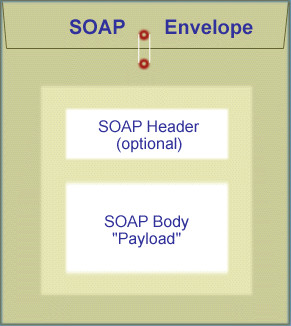
\includegraphics[scale=0.4]{soap_envelope.jpg}\\
  \caption{SOAP Envelop}
  \label{fig:soap_env}
\end{figure}

\paragraph{SOAP Message Example:}

The following example gives an overview of a SOAP message:

\lstset{language=XML}
\begin{lstlisting}
<?xml version="1.0"?>
<soap:Envelope xmlns:soap="http://www.w3.org/2003/05/soap-envelope">
  <soap:Header>
  </soap:Header>
  <soap:Body>
    <m:GetStockPrice xmlns:m="http://www.example.org/stock">
      <m:StockName>IBM</m:StockName>
    </m:GetStockPrice>
  </soap:Body>
</soap:Envelope>
\end{lstlisting}

\subsection{REST\label{sec:back_tech_ws_rest}}
In addition to SOAP, there is another alternative for the implementation of Web services. \citeauthor{Fielding2000} in his dissertation describes an architectural style that he calls REpresentational State Transfer architecture or short REST.

REST is based on principles that are used in the largest distributed application - the World Wide Web. The World Wide Web is itself a gigantic REST application. Many search engines, shops or booking systems have unintentionally been based on REST web services.

The REpresentational State Transfer Architecture is an architectural model, which describes how the Web should work. The model will serve as a guide and reference for future enhancements.

REST is not a product or standard. REST describes how web standards in a Web-friendly manner can be used.


\paragraph{REST Example:} An online store will serve here as an example of a RESTful application. In this application, there are customers who can place items in shopping carts.

Each object of the application, such as the product or the customer is a resource that is externally accessible via a URL. With the following request in the example application, the shopping cart with the number 7621 is retrieved.

%\lstset{language=JSON}
\begin{lstlisting}
GET /cart/7621
\end{lstlisting}

It is not specified in REST how the result of a request is represented. Client and server must have a shared understanding how the data is represented, i.e. in XML or JSON TODO akro. The following example is a response in JSON format.

%\lstset{language=JSON}
\begin{lstlisting}
{
"customer": 7621,
"articles":[
	{"position":1,
	"articleNumber"=89,
	"description":"iPhone5",
	"price":200},
	{"position":2,
	"articleNumber"=76,
	"description":"Samsung Galaxy S III",
	"price":150}
]
}
\end{lstlisting}

\subsection{SOAP vs. REST TODO\label{sec:back_tech_ws_rest}}

The main advantages of REST web services is that they are lightweight, without a lot of extra XML markup. Also REST has easy to read results and is easy to build requiring no special tool-kits.

SOAP also has some advantages, usually it is easy to use, provides relatively strong typing since it has a fixed set of supported data types, furthermore many different kinds of development tools are available.

Next some aspects of SOAP and REST will be compared.

\paragraph{API Flexibility \& Simplicity}

The key to the REST methodology is to use an interface that is already well known and widely used, the URI, in order to write web services. For example, providing a currency converter service, in which a user types-in the desired currencies for input and output and the specific amount in order to receive a real-time conversion, could be as simple as making a script accessible on a Web server via the following URI: http://www.currencyconverter.com\/convert?in=us-dollar\&value=100\&out=euro

This service could easily be requested with an HTTP GET command by any client or server application with HTTP support. The resulting HTTP response depends on how the service provider wrote the script and it might be as simple as some standard headers and a text string containing the current price for the given currencies, or it might be an XML document.
\\
\\
The significant advantages of this interface method over SOAP-based services are as follows:-
\\
\\
The creation and modification of a URI in order to access different web resources can easily be figured out by any developer. However, in order for SOAP to be used, most developers would need a SOAP toolkit to form requests and obtain the results, as it requires specific knowledge of a new XML specification.
\\
\\
\paragraph{Bandwidth Usage}

The RESTful interface has short requests and responses, which is another advantage. Whereas, an XML wrapper around every request and response is required for SOAP. For a four- or five-digit stock quote, a SOAP response may require more than 10 times the number of bytes as the same response in REST, as SOAP requires namespaces and typing to be present. 
\\
\\
\paragraph{Security}
The security perspective debate is probably the most interesting aspect of the comparison between REST and SOAP. 

Sending remote procedure calls (RPC) through standard HTTP ports is seen by the SOAP camp as being a good way to ensure Web services support across organizational boundaries. In contrast however, REST followers see this as compromising network safety and considers this practice a major design flaw.

With REST, the administrator (or firewall) can discern the intent of each message by analyzing the HTTP command used in the request, even though the REST calls also go over HTTP or HTTPS. For example, a GET request is always seen as being safe because by definition, the data cannot be modified. It can only query data.

On the other hand, HTTP POST is used by a typical SOAP request to communicate with a given service. Without looking into the SOAP envelope, it is not possible to know whether the request simply wants to query data or delete entire tables from the database. This task is resource-consuming and it is not built into most firewalls.

On the downside with SOAP, the difficult task of authentication and authorization is left up to the application developer. However, the fact that the web servers already have support for these tasks, is taken into account by the REST methodology. REST methodology developers can make the network layer do all the heavy work by using industry-standard certificates and a common identity management system, such as an LDAP server.

However, REST is not perfect. It is not always the best solution for every web service. Data should never be sent as parameters in URIs in order to be kept secures. 

\paragraph{Type Handling}

Due to its fixed set of supported data types, SOAP provides a stronger typing. In this way, it ensures a return value  will be given in the corresponding native type in a specific platform. For example, when an API is HTTP based, the return value will need to be deserialized from its original XML format before being type-casted.    
However, handling complex data-types proves to be the main challenge and is mainly achieved by defining a serialization and deserialization mechanism, wherefore there is no definitive advantage concerning ease of client-side coding. 


\paragraph{Client-side Complexity}

Making calls to an REST API poses less of a challenge than making calls to a SOAP API. While REST is elementary to all programming languages and merely implies constructing an HTTP request with the appropriate parameters, the latter requires a client library, a Stub and involves additional learning effort.  

\paragraph{Testing and Troubleshooting}

A further characteristic of REST APIs is their easy testing and troubleshooting ability, requiring no more than a browser, the response appearing in the browser window itself. Generating a request does not require special test tools, this is a major advantage of REST based APIs.  
  

\paragraph{Server-side Complexity}

The majority of programming languages provide easy to operate mechanisms to expose a method using SOAP. However exposing a method using REST based APIs, involves additional effort due to the task of mapping the URI path to specific handlers. Though various frameworks facilitate this task, the exposition of methods is still easier to achieve using SOAP than REST.

\paragraph{Caching}

To consume a REST based API service, a simple GET request is needed, therewith allowing proxy servers to cache their response very easily. In contrast, SOAP requests use POST and require a complex XML format, producing difficulties for response-caching.

\subsection{NoSQL Databases TODO NoSQL Evaluation\label{sec:back_da_per}}
SQL databases have been used to solve storage problems for a long time, including cases in which there is a high discrepancy between the object model and its relational model. The conversion of graphs to tables represents yet another dis-functional use of data mapping. The complex structure this sort of mismanagement causes depends on mapping frameworks and complex algorithms. The rigid relational scheme characteristic for SQL becomes especially inefficient for such web applications as blogs due to their multifaceted range of attributes that need to be stored in their respective tables, e.g. comments, pictures, audios, videos, source codes. Therefore adding or removing a new feature to this sort of website will necessarily result in system unavailability.          

Nowadays of course,  web sites are developing towards more interactive models, obliging databases to perform real-time scheme updates, thereby paving the way for NoSQL TODO akr to provide a database molded for modern demands. %The following section describes the characteristics of NoSQL and its different types of databases.   

%\subsubsection{SQL\label{sec:back_da_per}}
%\subsubsection{NoSQL\label{sec:back_da_per}}	

There is a variety of ideas surrounding the NoSQL movement, however the core idea is to provide more flexible data models, as opposed to the SQL approach, in order to provide live scheme updates. The ever increasing amount of data streaming through the web implies challenges, which any competitive website wishing to stay in business will have to meet. Besides dealing with vast amounts of data, these sites have to respond to constant requests around the globe without allowing any noticeable latency.

To this end, many companies have developed their own storage systems, according to their specific needs, which have been classified as NoSQL databases. Considering the fact that these stores are set up to fulfill the individualized requirements of the companies they belong to, there can be no final answer as to which of them  works most efficiently. For example, Facebook implemented the NoSQL database Cassandra in order to solve the so called "Inbox Search Problem" - the challenge of allowing Facebook users to search through their sent and received messages - caused by the multitude of stored data alongside the high number of active users. 

The following sections will examine the structure and flexibility of four different data models offered by NoSQL systems, each accompanied by one or more exemplary implementations.      

\subsection{Key Value Stores}
Key value stores are similar to maps or dictionaries where data is addressed by a unique key. 

Key value stores are useful for simple operations, which are based on key attributes only. In order to speed up a user specific rendered webpage, parts of this page can be calculated before and served quickly and easily out of the store by user IDs when needed. Since most key value stores hold their dataset in memory, they are oftentimes used for caching of more time intensive SQL queries. Key value stores considered in this paper are Project Voldemort [6], Redis [7] and Membase [8].


\subsection{Document Stores}
Document Stores encapsulate key value pairs in ISDN or ISDN like documents. Within documents, keys have to be unique. Every document contains a special key "ID", which is also unique within a collection of documents and therefore identifies a document explicitly. In contrast to key value stores, values are not opaque to the system and can be queried as well. Therefore, complex data structures like nested objects can be handled more conveniently. Storing data in interpretable ISDN documents have the additional advantage of supporting data types, which makes document stores very developer-friendly. Similar to key value stores, document stores do not have any schema restrictions. Storing new documents containing any kind of attributes can as easily be done as adding new attributes to existing documents at runtime.

Document stores offer multi attribute lookups on records which may have complete different kinds of key value pairs. Therefore, these systems are very convenient in data integration and schema migration tasks. Most popular use cases are real time analytics, logging and the storage layer of small and flexible websites like blogs. The most prominent document stores are CouchDB [9], MongoDB [10] and Riak [11].

\subsection{Column Stores}
Column Family Stores are also known as column oriented stores, extensible record stores and wide columnar stores. All stores are inspired by Googles Bigtable [12], which is a "distributed storage system for managing structured data that is designed to scale to a very large size" [12]. Bigtable is used in many Google projects varying in requirements of high throughput and latency-sensitive data serving. The data model is described as "sparse, distributed, persistent multidimensional sorted map" [12]. In this map, an arbitrary number of key value pairs can be stored within rows. Since values cannot be interpreted by the system, relationships between datasets and any other data types than strings are not supported natively. Similar to key value stores, these additional features have to be implemented in the application logic. Multiple versions of a value are stored in a chronological order to support versioning on the one hand and achieving better performance and consistency on the other one (chapter four). Columns can be grouped to column families, which is especially important for data organization and partitioning (chapter five). Columns and rows can be added very flexibly at runtime but column families have to be predefined oftentimes, which leads to less flexibility than key value stores and document stores offer. HBase [13] and Hypertable [14] are open source implementations of Bigtable, whereas Cassandra [15] differs from the data model described above, since another dimension called super columns is added. These super columns can contain multiple columns and can be stored within column families. Therefore Cassandra is more suitable to handle complex and expressive data structures.

\subsection{Graph Stores:}


\subsection{Application Messaging\label{sec:back_me_mid}}
	
\subsection{Search Engines \label{sec:back_se_en}}
\subsubsection{Apache Solr \label{sec:back_se_solr}}
\subsubsection{Elasticsearch \label{sec:back_se_es}}
			
\subsection{Web Servers\label{sec:back_we_se}}
\subsubsection{Apache \label{sec:back_ap}}
\subsubsection{NginX\label{sec:back_ng}}

\subsection{Spring Framework\label{sec:back_sp_fr}}

\subsection{Application Servers\label{sec:back_sp_fr}}

\section{Related Work\label{sec:back_rel_work}}